\chapter{Model Development}\label{ch:model_development}
One of the goals for this project was to research, design and compare different neural network topologies. 
Some of these were feed-forward and recurrent.
Continuing, some neural networks were made deep, first by adding fully connected layers to the existing type feed-forward, CNN or RNN.
Different configurations were tested, some proving to be efficient for achieving designated goals, and some less so.
Subject to further research, we found that recurrent neural networks work best for speech recognition.
Therefore  the following comparison will be based on different RNNs configurations.\\\\

\section{Neural Network Comparison}\label{sec:NNComparison}

In this chapter two models are developed based on the simple LSTM model from the silicon-valley-data-science RNN tutorial \cite{rubashkin2017}. Firstly these models (including "their simple LSTM model") will be trained and tested on a small data set with the numbers:\\\\
$\left\{zero, one, two, three, four, five, six, seven, eight, nine \right\}$,\\\\
the same data used in Chapter \ref{ch:machine_learning} for the parameter comparison. After that, the best performing model shall be picked for a more detailed description (with code) and further training with a bigger data set of the English language.\\\\
Before the comparison of the 3 models, lets take a look at their structure in the following diagrams.
As mentioned earlier the two models that were developed are based on the silicon-valley-data-science simple LSTM model. Their model consist of two LSTM layers as shown in the diagram below (Figure \ref{fig:simple_LSTM}).
\begin{figure}[H]
	\centering
	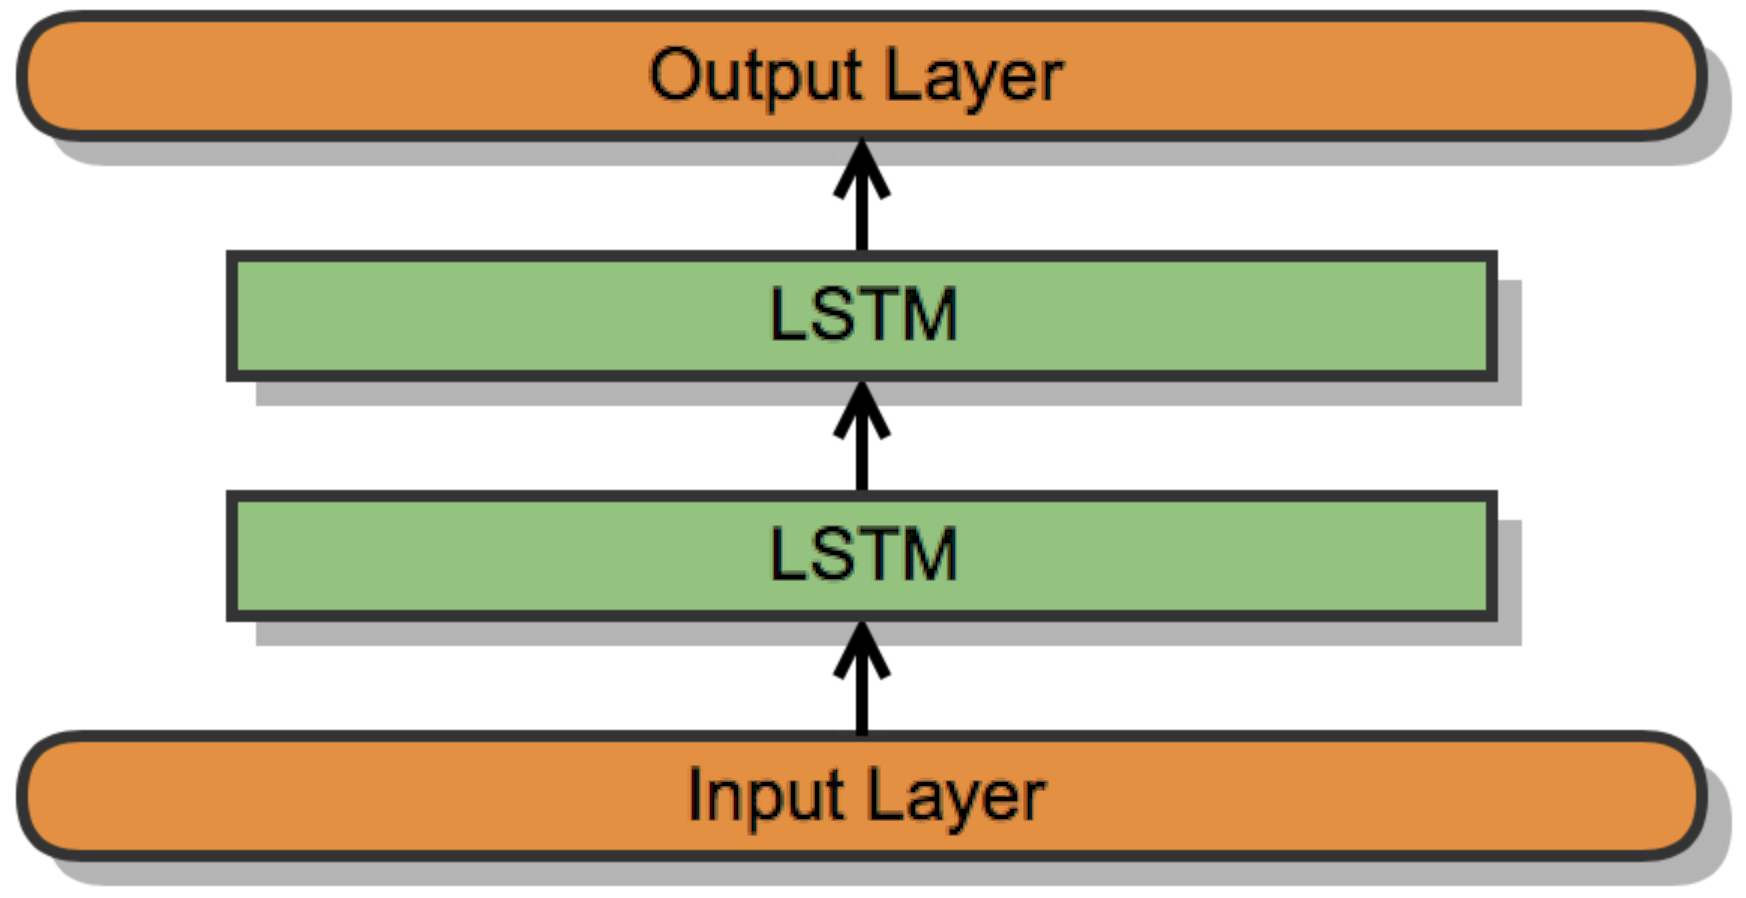
\includegraphics[width=.35\textwidth]		
	{model_development/01_simpleLSTM}
	\caption{Simple LSTM model.}
	\label{fig:simple_LSTM}
\end{figure}
Based on model above, it was decided among us to make an addition of two fully connected (FC) layers before and one FC layer after the two LSTM layers (shown in Figure \ref{fig:simple_LSTMFC}), with the desire of gaining better accuracy.
\begin{figure}[H]
	\centering
	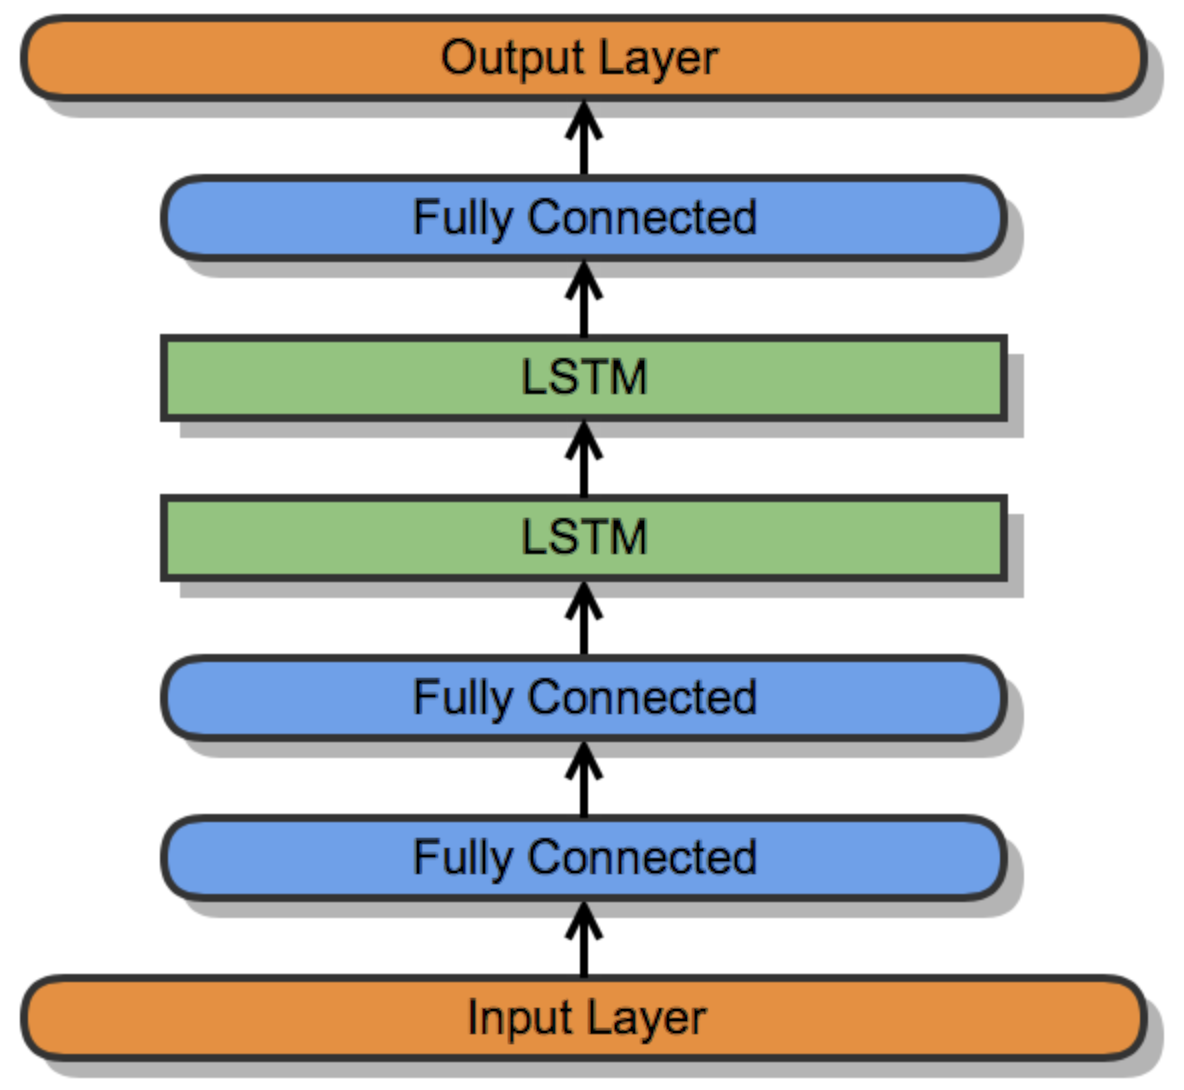
\includegraphics[width=.35\textwidth]		
	{model_development/02_simpleLSTMFC}
	\caption{Simple LSTM model with fully connected layers.}
	\label{fig:simple_LSTMFC}
\end{figure}
After that, a decision was made to replace the to LSTM layers in the model above with one Bi-Directional LSTM layers (seen in Figure \ref{fig:BiRNNFC}), again with the desire to make a more accurate model
\begin{figure}[H]
	\centering
	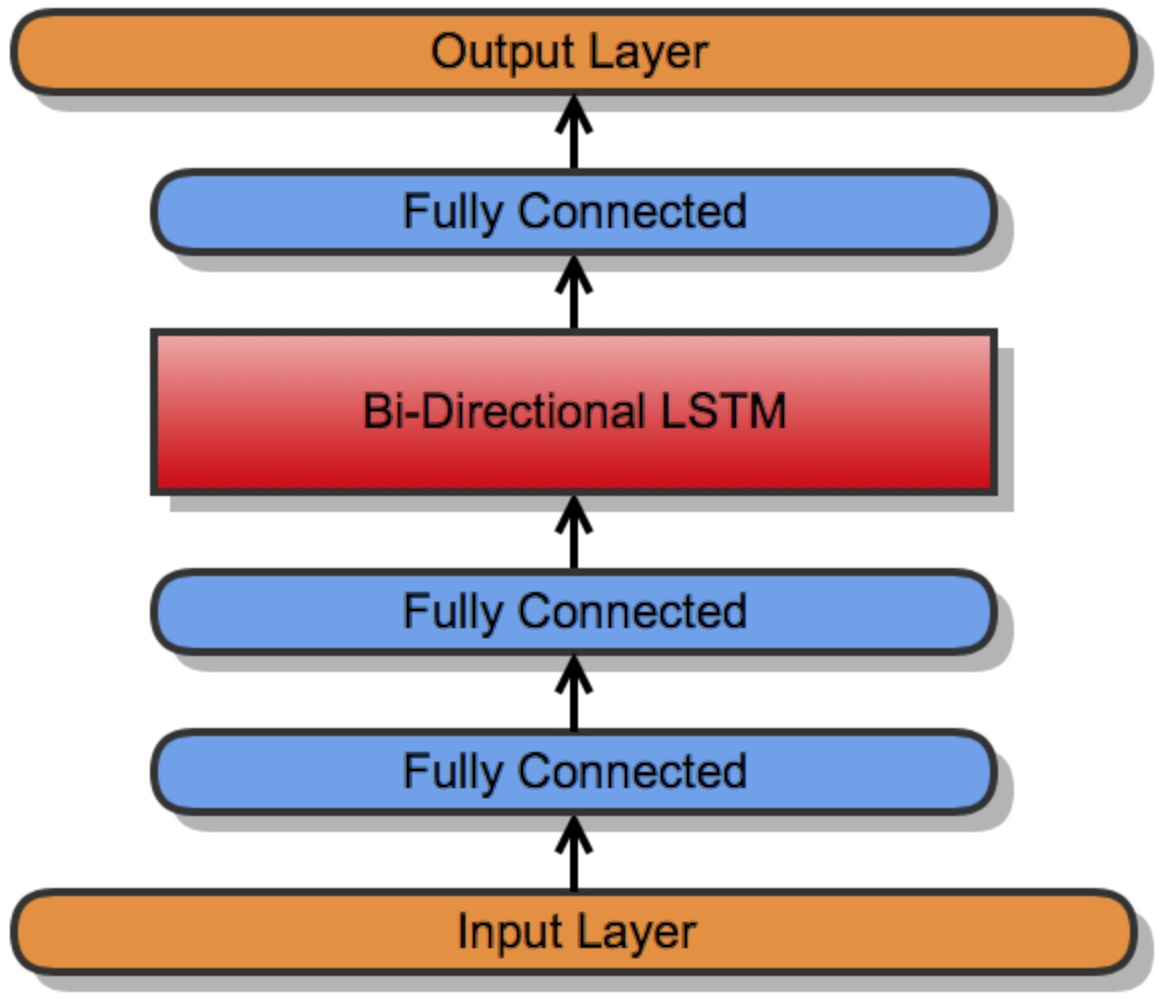
\includegraphics[width=.35\textwidth]		
	{model_development/03_BiRNN}
	\caption{BiRNN model with fully connected layers.}
	\label{fig:BiRNNFC}
\end{figure}

In order to have a fair comparison between these model the parameters values were made to be the same for all models as shown in Table \ref{tab:3models_tab}.
The respective models are mapped to the described ones in Table \ref{tab:3_models}. For the interested reader an expanded version in appendix \ref{ch:appClabel}.
\begin{table}[H]
\centering
    \caption{Parameter values of the three model.}
    \begin{tabular}{| l | c | c | c | c |} 
    \hline
        Parameters & 
        Model1 -\tikzcircle[pink, fill=pink]{3pt}- &
        Model2 -\tikzcircle[red, fill=red]{3pt}- &
        Model3 -\tikzcircle[turquoise, fill=turquoise]{3pt}-\\
    \hline
        Batch Size & 
        50 \hfill 20 \hfill 20 & 
        50 \hfill 20 \hfill 20 & 
        50 \hfill 20 \hfill 20 \\
    \hline
        Dropout & 
        0.05 & 0.05 & 0.05 \\
    \hline
        Learning Rate & 
        0.001 & 0.001 & 0.001 \\ 
    \hline
    \end{tabular}
    \label{tab:3models_tab}
\end{table}
\begin{table}[H]
\centering
	\caption{Models.}
	\begin{tabular}{ l  c }
	Model1 -\tikzcircle[pink, fill=pink]{3pt}- &
	(simple LSTM Model)\\
	Model2 -\tikzcircle[red, fill=red]{3pt}- &
	(simple LSTM + FC Model)\\
	Model3 -\tikzcircle[turquoise, fill=turquoise]{3pt}- &
	(BiRNN + FC Model)\\
	\end{tabular}
	\label{tab:3_models}
\end{table}

The following graph (Fig. \ref{fig:test_error_fig}) and
table (Tab. \ref{tab:test_error_tab}) represent the error
rate for the test data set. The results show that Model1 has $\sim 20\%$ word error rate (WER) while
Model2 and Model3 is $\sim 8\%$ and $\sim 0\%$ WER respectively.

\begin{figure}[H]
	\centering
	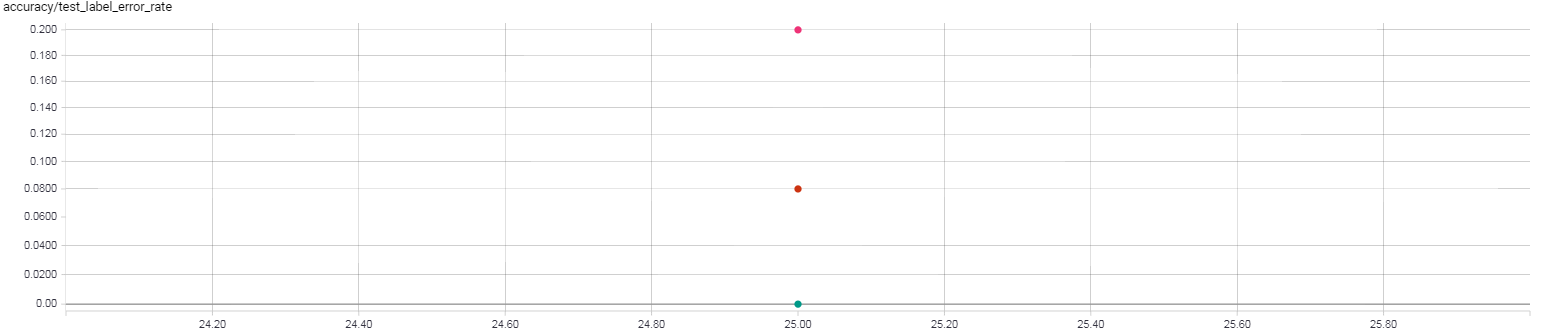
\includegraphics[width=\textwidth]		
	{model_development/3models_comparison/test_error_rate_3models}
	\caption{Test error rate.}
	\label{fig:test_error_fig}
\end{figure}

\begin{table}[H]
\centering
	\caption{Test error rate results.}
	\begin{tabular}{| l | c | c | c |}
	\hline
	Models & Value & Epoch & Duration \\
	\hline
	Model1 -\tikzcircle[pink, fill=pink]{3pt}- &
	0.200 & 25.00 & 0s\\
	\hline
	Model2 -\tikzcircle[red, fill=red]{3pt}- &
	0.080 & 25.00 & 0s\\
	\hline
	Model3 -\tikzcircle[turquoise, fill=turquoise]{3pt}- &
	0.000 & 25.00 & 0s\\
	\hline
	\end{tabular}
	\label{tab:test_error_tab}
\end{table}

The following graph (Fig. \ref{fig:validation_error_fig}) and
table (Tab. \ref{tab:validation_error_tab}) represent the error
rate for the validation data set. The results show that Model1 has took $\sim 7m 9s$ to complete training while
Model2 and Model3 is $\sim 9m 8s$ and $\sim 11m 49s$ respectively.

\begin{figure}[H]
	\centering
	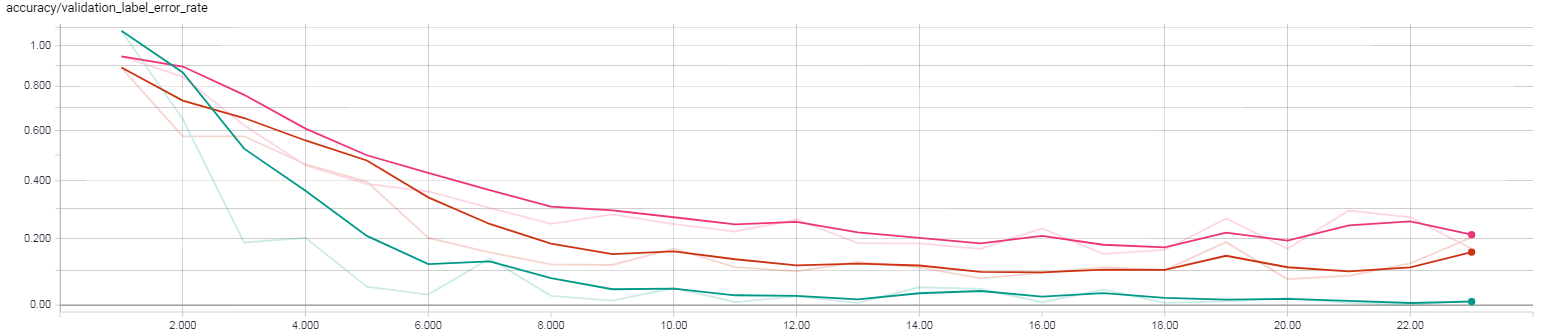
\includegraphics[width=\textwidth]		
	{model_development/3models_comparison/validation_error_rate_3models}
	\caption{Validation error rate.}
	\label{fig:validation_error_fig}
\end{figure}

\begin{table}[H]
\centering
	\caption{Validation error rate results.}
	\begin{tabular}{| l | c | c | c |}
	\hline
	Models & Value & Epoch & Duration \\
	\hline
	Model1 -\tikzcircle[pink, fill=pink]{3pt}- &
	0.1669 & 23.00 & 7m 9s\\
	\hline
	Model2 -\tikzcircle[red, fill=red]{3pt}- &
	0.2030 & 23.00 & 9m 8s\\
	\hline
	Model3 -\tikzcircle[turquoise, fill=turquoise]{3pt}- &
	0.01398 & 23.00 & 11m 49s\\
	\hline
	\end{tabular}
	\label{tab:validation_error_tab}
\end{table}

The final results show that Model1 was improved by adding the fully connected layers (Model2) from $\sim 20\%$ to $\sim 8\%$ WER and further improved by the replacing the two LSTMs by one Bi-Directional LSTM layer (Model3) from $\sim 8\%$ to $\sim 0\%$ WER.
The graph for the validation error rate (Figure \ref{fig:validation_error_fig}) clearly shows the three distinct lines in "parallel" with each other. The top line being the least accurate and the bottom one being the most.

\section{Model Description}

Model3 (BiRNN) is better therefore we go into more detail about it...

As shown in Subsection \ref{sub:BiRNN}, the model that is used in this DSR system is a recurrent neural network.
This recurrent network is based on the standard TensorFlow implementation of an LSTM cell, called "BasicLSTMCell", and used as a bidirectional layer. 
There are two cells in the layer, one "forward" direction and one "backward" direction.
Each cell is unrolled 1024 times, giving the layer 2048 elements. 
The purpose is to recognize the context of the text, thus improving the prediction accuracy.
The complete topology for the network is as follows: \\\\
\todo{Make full page png}
\begin{figure}[H]
	\centering
	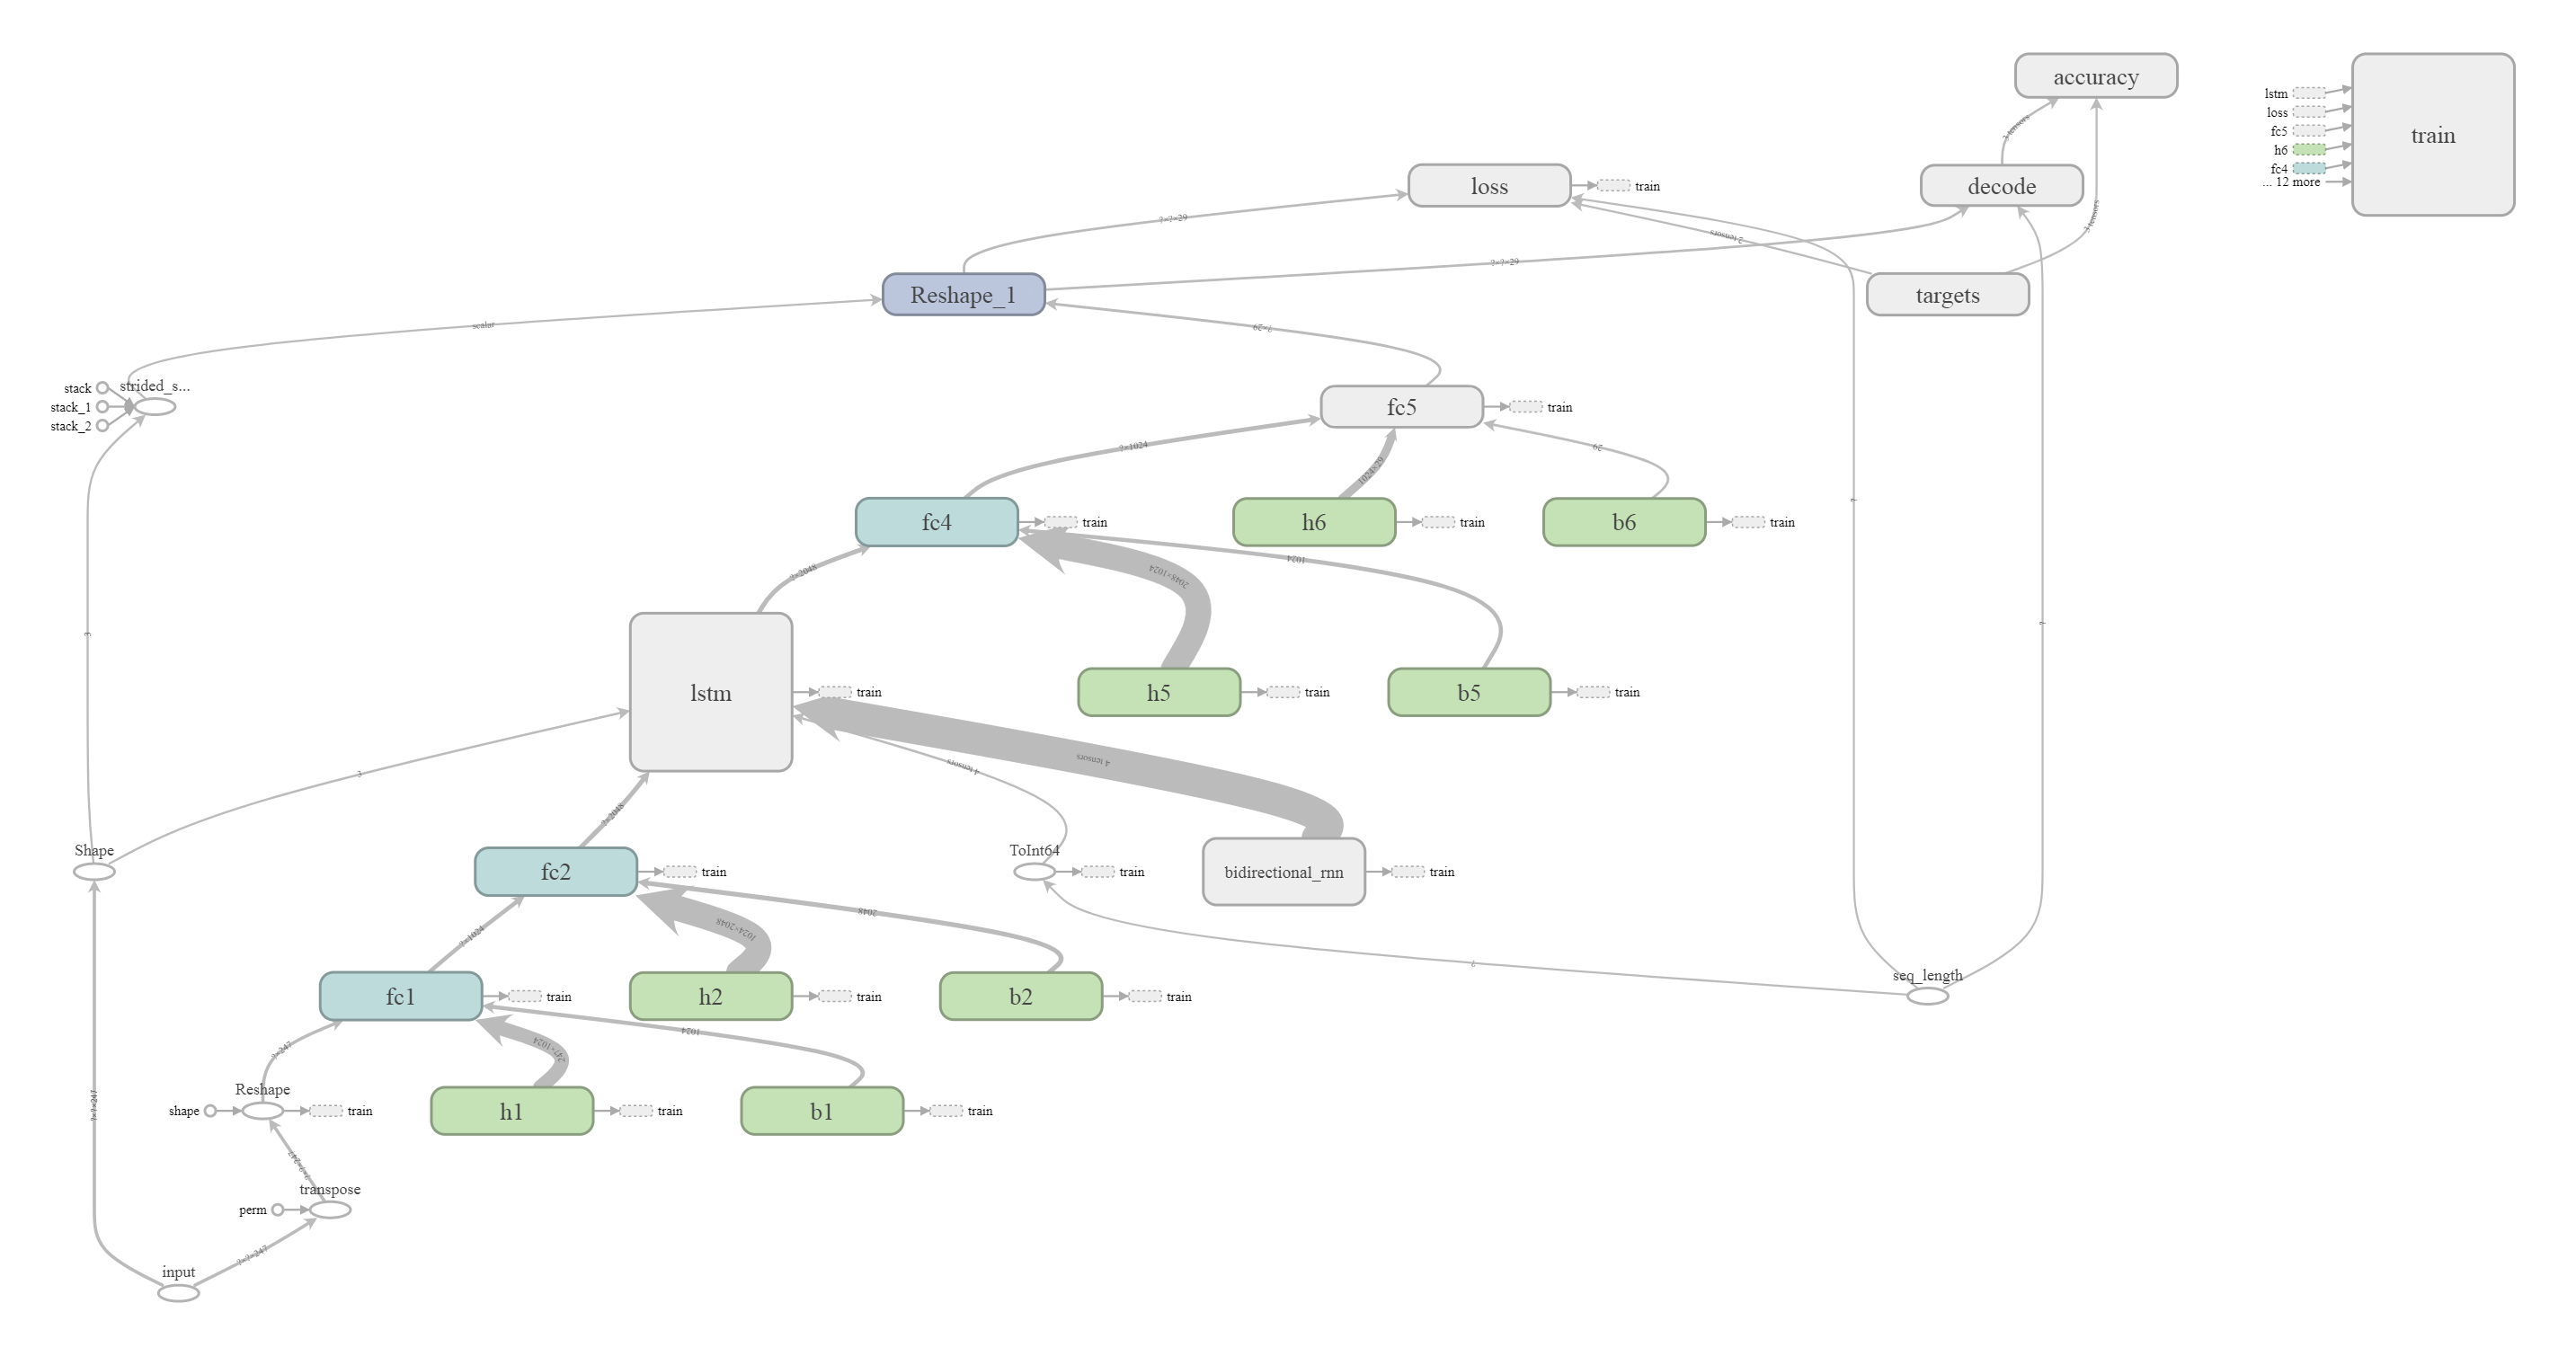
\includegraphics[width=\textwidth]		
	{model_development/birnn_v2_graph}
	\caption{Our BiRNN model graph.}
\end{figure}
Figure X shows the complete topology of the network used in the current implementation.
The structure is: 2-BiRNN-1-output.
In the beginning there are 2 fully connected layers, each consisting of 1024 neurons.\\
The first layer is designed to accept input from a 2D tensor. However, the input tensor has 3 dimensions.
To resolve this discrepancy, the input tensor is reshaped into a 2D representation. Two dimensions are merged, thus the 3D tensor becomes 2D, and is ready to be sent through the network.
After the multiplication, the activation function is applied. 
For this type of layer, ReLU activation is used. 
The last operation in the layer applies drop-out on the neurons.
To visualize elements over time, TensorFlow's TensorBoard utility is used, and various information is saved after every layer.
\lstinputlisting[language=Python,caption = First fully connected layer, firstline=657, lastline=667]{code/rnn.py}
The second layer has much of the same functionality as the first. However, they differ in the output dimension size, because the output of this layer is going to be the input for the bidirectional LSTM layer.
\lstinputlisting[language=Python,caption = Second fully connected layer, firstline=669, lastline=678]{code/rnn.py}
The next layer defines two LSTM cells. Both are initialised with the default forget bias, in order to remember more information at the beginning of training. For these cells there is no drop-out.
\lstinputlisting[language=Python,caption = BiRNN Layer, firstline=694, lastline=702]{code/rnn.py}
Further on, the input is reshaped into a three dimensional tensor, to be compatible with the BiRNN layer, and the network is unrolled. 
\lstinputlisting[language=Python,caption = BiRNN Layer, firstline=718, lastline=723]{code/rnn.py}
Following, the previous outputs is reshaped again into a 2 dimensional tensor, and sent to the next fully connected layer. 
This layer is similar to the first two, with the main operation being tensor multiplication and addition.
Afterwards, ReLU and drop-out is applied.
\lstinputlisting[language=Python,caption = Third fully connected layer, firstline=732, lastline=737]{code/rnn.py}
The output layer, is used as the end point of the network.
Multiplication and addition operations are applied to the previous output tensor. 
At this point, the output was  transformed by the entire network. 
The last step is to reshape the tensor back into a 3D form, after which it is passed to another function for decoding.
\lstinputlisting[language=Python,caption = Output layer, firstline=746, lastline=748]{code/rnn.py}
